\section{Introduction}

Renewable energies are currently advancing and gaining an increasing share of the energy production. On the one hand, this is induced by the desire to decrease the carbon footprint and on the other hand, the population is facing a decreasing availability of fossil fuels like natural gas, coal and oil. The advantage of renewable energies is that apart from not requiring fuel, which induces zero fuel costs, it is emission-free and therefore supported by the government. However, these energy sources are also non-dispatchable and have the major disadvantage of uncertainty. Conejo et al. \cite{Conejo10} considered the case of a wind power producer. Due to the uncertainty, the wind power producer must rely on the energy traded on the balancing market. Therefore, he solved an optimisation problem to maximise the expected profits from trading on the day-ahead market and the adjustment market while also minimising the costs incurred in the balancing market caused by energy deviations. 

In addition to the uncertainty, the wind power producer also faces a substantial fluctuation in production throughout the year, caused by the strong dependence on wind availability over different months in a year. Considering a wind power producer in Europe, wind availability is much higher in the winter than summer months, see, e.g. \cite{W11}. 

For this case study, we consider the case of an energy producer producing both wind power as well as solar energy. Several studies have been carried out to see how both resources' production variability  can be decreased by exploiting the anti-correlation of wind speed and solar irradiance. Coker et al. \cite{Coker2013} considered a region in south-west Britain to assess the variability of wind, solar and tidal current energy resources. Santos-Alamillos et al. \cite{Santos-Alamillos} aimed at finding the optimal spatial distribution of wind and solar farms across the Southern Iberian Peninsula to minimise the resulting net variability. Bett et al. \cite{BETT16} analysed daily data for Great Britain and found  evidence for an overall anticorrelation between wind speed and solar irradiance. As a side product, they also discovered that solar variability is significantly higher than wind variability and that both variabilities are higher in winter than in summer. Inspired by these results, we wish to set up a pool trading model for an energy producer offering energy produced from both solar and wind power plants.  
This setting of a hybrid wind-solar power producer
	overcomes the strong fluctuation in production throughout the year due to the strong over year anti-correlation of wind speed and solar irradiance, see figure \ref{fig:overyear}. In addition to
	the anti-correlation between wind speed and solar irradiance over the whole year, there is also an anti-correlation between both over the day, even if it is much smaller. We will exploit this anti-correlation over the day and include it into the forecast
	for wind and solar power production. Therefore, we will apply the forecast for wind power production for a time $t$ in dependence on the previous times' wind speeds and previous times' solar irradiance to improve the forecast precision possibly.
	\laura{Brauchen wir (a) und (b) und warum ist die y-Achsen Beschriftung nur rechts?}
	
\begin{figure}[h!]
	\centering
	
	\begin{minipage}{0.8\textwidth}
		\subfloat[]{
			\centering
			\scalebox{0.4}{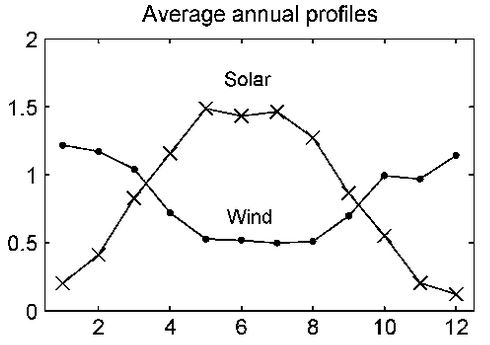
\includegraphics{Figures/year.jpg}}
		}
		\hfill
		\subfloat[]{
			\centering
			\scalebox{0.4}{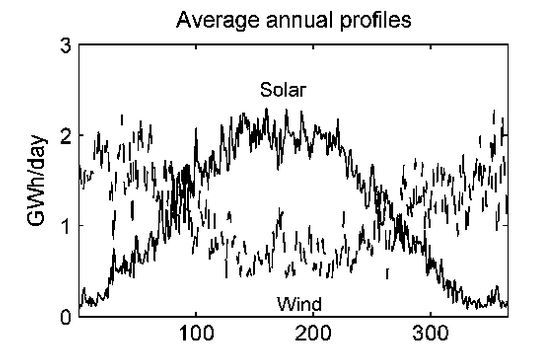
\includegraphics{Figures/year2.png}}
		}
		
		\caption{The average annual profiles of solar irradiance and wind speed \cite{W11}}\label{fig:overyear}
	\end{minipage}	
\end{figure}
To solve the  decision problem, the hybrid energy producer has to face, we will solve a scenario-based multi-stage optimization problem. For generating wind and solar power scenarios, we will use a time-series-based approach. With the generated data, we consider two cases. First, we look at a situation where we do not have an adjustment market. Second, we add an adjustment market to our situation. We compare the revenue of a hybrid producer with the sum of the revenues of a solar and a wind power producer. Our results show that the more risk averse a producer is, the more profitable it is to produce in a hybrid scheme. This effect can be observed in both market situations. We conclude that this profitability stems from the anit-correlation of the two weather conditions as a decrease in availability of solar irradiance is most likely to be compensated by an increase of wind speed and vice versa. This gives more planning security and therefore a higher expected profit. Moreover, the decrease in planning insecurity also explains why more risk averse producers profit more from a hybrid production scheme.  
